% !Tex root = Vorlage.tex
\newpage
\section{Execution}
A number of experiments have been conducted in order to evaluate the capabilities of empirical risk minimization (ERM) techniques for functional dependency discovery.

\subsection{FD Imputer}
The FD Imputer

\subsection{ML Imputer}

\subsubsection{Overfitting the ML Imputer}

\subsection{Comparing ML Imputer with FD Imputer}
When comparing the ML Imputer to the FD Imputer, it is necessary to explain the scope of such an comparison.
Due to the definition of a FD, the FD Imputer cannot approximate numerical values.
Meanwhile, the ML Imputer is able to do so due to the approximative nature of a classifier.
To compare classification performance,

\begin{figure}[h]
     \centering
     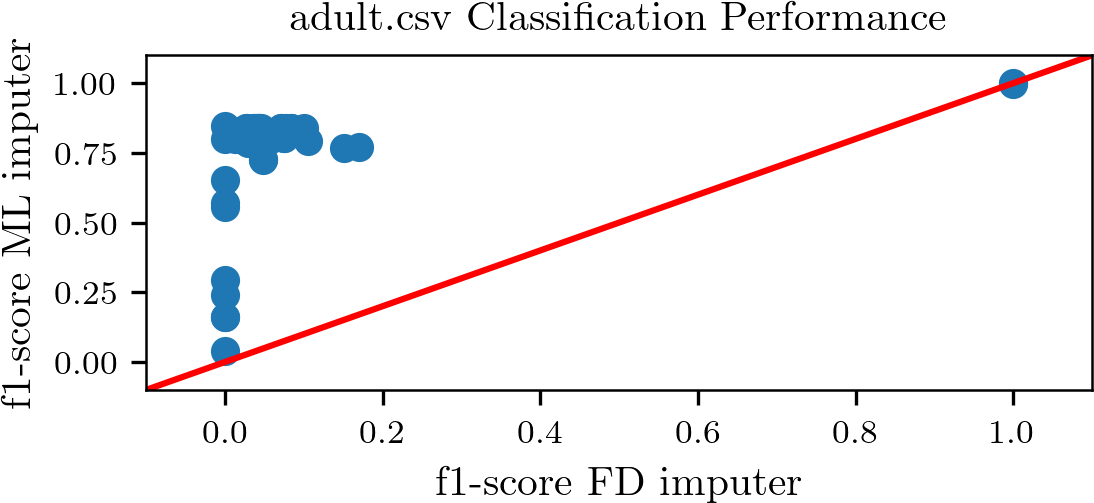
\includegraphics[width=.8\textwidth]{../figures/adult/f1_ml_fd_adult}
     \caption{The figure compares the f1-score of the FD Imputer compared to the f1-score of the ML Imputer. Each point represents one left-hand side.}
     \label{fig:f1_ml_fd_adult}
 \end{figure}

 \begin{figure}[h]
     \centering
     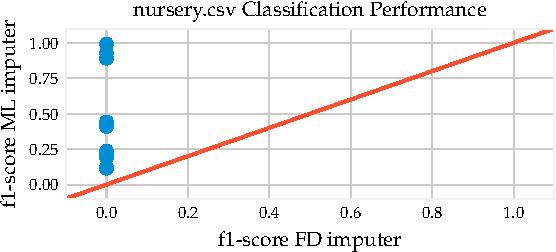
\includegraphics[width=.8\textwidth]{../figures/nursery/f1_ml_fd_nursery}
     \caption{Some ohter caption.}
     \label{fig:f1_ml_fd_nursery}
\end{figure}

\subsection{Begriffsdiskussion}
Lorem ipsum dolor sit amet, consetetur sadipscing elitr, sed diam nonumy eirmod
tempor invidunt ut labore et dolore magna aliquyam erat, sed diam voluptua. At
vero eos et accusam et justo duo dolores et ea rebum. Stet clita kasd gubergren,
no sea takimata sanctus est Lorem ipsum dolor sit amet.
